\documentclass[fontsize=11pt]{article}
\usepackage{amsmath}
\usepackage[utf8]{inputenc}
\usepackage[margin=0.75in]{geometry}
\usepackage{url}
\usepackage{enumitem}
\usepackage{graphicx}
\title{CSC111 Final Report: The National Basketball Association's Statistically Best Players}
\author{Junwei Quan, Vincent Louie}
\date{Saturday, April 1, 2023}

\begin{document}
\maketitle

\section{Introduction}

\hspace{\parindent{}} 
The National Basketball Association (NBA) is one of the most popular professional sports leagues in the world. Throughout its history, countless talented players have graced the courts and entertained millions of fans. One of the key aspects of any professional sport is the recognition of exceptional talent through awards. The NBA has several awards that recognize various achievements, such as Most Valuable Player (MVP), Rookie of the Year, and Defensive Player of the Year, among others.\\

Given the vast number of players and awards, it becomes an interesting challenge to analyze the relationships between players and their achievements throughout their careers. To address this challenge, our project aims to create a visual representation of NBA players and their respective awards, enabling us to examine the correlations and draw insights from the data.\\

Our main goal is to create an "AwardNetwork" using Python programming that represents the connections between NBA players and the awards they have achieved. This network will be visualized using graphs, allowing us to easily explore the relationships between players and their awards. By examining the AwardNetwork, we hope to answer questions such as:\\

\begin{itemize}
    \item Which players have the most awards, and how do their careers compare to others?
    \item Are there any commonalities among players who have won specific awards?
\end{itemize}

To achieve our goal, we will use a dataset containing information on the top 80 NBA players and their awards, along with relevant background information such as age, career duration, and Hall of Fame status. We will then implement various Python classes and methods to parse the data, construct the AwardNetwork, and visualize the graph using libraries such as NetworkX, Plotly, and Matplotlib.\\

\textbf{Ultimately, our project aims to provide a deeper understanding of the achievements of NBA players and the role that awards play in shaping their careers. We believe that this analysis will not only be of interest to basketball enthusiasts but also contribute to the broader understanding of performance recognition in professional sports.}

\section{Datasets description}
In this study, we utilize two distinct datasets to analyze and compare the performance and achievements of players.
\subsection{Official NBA Dataset}
The first dataset is sourced from RealGM and we did some addition research to combine the dataset with age, status, year and some factors we have as the attributes of our class, which provides a comprehensive overview of individual player statistics and awards they have. Some of the awards and distinctions covered in the dataset include the Michael Jordan Most Valuable Player (MVP), Bill Russell NBA Finals MVP, All-NBA First Team, Hakeem Olajuwon Defensive Player of the Year and many others. This dataset offers a detailed overview of the players' accomplishments and provides valuable insights into their impact on the sport. The dataset also includes the name of the image icon that is associated to the specific player which is used in the visualization process.
\subsection{Custom Awards Points Dataset}
The second dataset is a custom creation that focuses on quantifying the value of various awards earned by NBA players throughout their careers.By assigning specific point values to each award, we aim to provide a comprehensive evaluation and comparison of player achievements. The point system takes into account the prestige and significance of each award, with more influential awards receiving higher point values.  The dataset also includes the name of the image icon that is associated to the specific player which is used in the visualization process.

\section{Computational Overview}

\hspace{\parindent{}} Our project uses various types of data to represent the NBA players and their awards. The primary dataset contains information on the top 75 NBA players, including their names, ages, career durations, Hall of Fame status, and the awards they have achieved. We utilize trees and graphs to represent the connections between players and the awards they have won, forming the basis of our AwardNetwork.

The major computations our program performs include:

\begin{enumerate}
    \item Data parsing and representation: We read data from CSV files (\texttt{player\_data.csv} and \texttt{award\_data.csv}) and store them in lists. We then create custom classes to represent the relevant domain entities, such as \texttt{BasketballPlayer}, \texttt{Award}, and \texttt{Achieved}. These classes help us model the relationships between players and awards, with the \texttt{Achieved} class acting as an edge in our graph.
    
    \item Building the AwardNetwork: We construct the AwardNetwork using the parsed data. Our \texttt{AwardNetwork} class contains methods to add players (\texttt{add\_players}), awards (\texttt{add\_awards}), and their achievements (\texttt{add\_achieves}). These methods utilize the \texttt{NetworkX} library to create nodes and edges, forming the graph.
    
    \item Data aggregation: We compute the total points for each player based on their awards using the \texttt{get\_total\_points} method in the \texttt{BasketballPlayer} class. This method calculates the total points for each player by multiplying the number of times they have won an award by the points associated with the award.
    
    \item Visualization: Our program reports the results of the computation by visualizing the AwardNetwork graph using the \texttt{NetworkX}, \texttt{Plotly}, and \texttt{Matplotlib} libraries. The \texttt{draw\_network} function takes the network and creates a \texttt{NetworkX} graph which is used as an input and generates a visual representation of the graph, with nodes representing players and awards, and edges representing the Achieved connections.
    
    \item Library usage: We utilize several libraries to accomplish the tasks mentioned above. The \texttt{NetworkX} library plays a central role in constructing the graph and performing graph-related computations. We use functions such as \texttt{add\_node}, \texttt{add\_edge}, and \texttt{spring\_layout} to create nodes, edges, and layout the graph. The \texttt{Plotly} and \texttt{Matplotlib} libraries are used to create the final visual representation of the graph, with functions such as \texttt{imshow}, \texttt{axis}, and \texttt{show} helping us display images, set axis properties, and present the graph.
\end{enumerate}

Our program effectively models the relationships between NBA players and their awards, providing valuable insights into the careers of these exceptional athletes. The use of trees and graphs, along with the appropriate libraries, allows us to parse, represent, and visualize the data in a meaningful and engaging manner.

\section{Instruction}

After downloading the ZIP file which includes everything needed for our program, ensure that everything from the requirements.txt is installed. After this, you will be able to run the main.py file which will give a new window which is our graphical user interface that is used to see the graph visualizations, which will look like this:\\
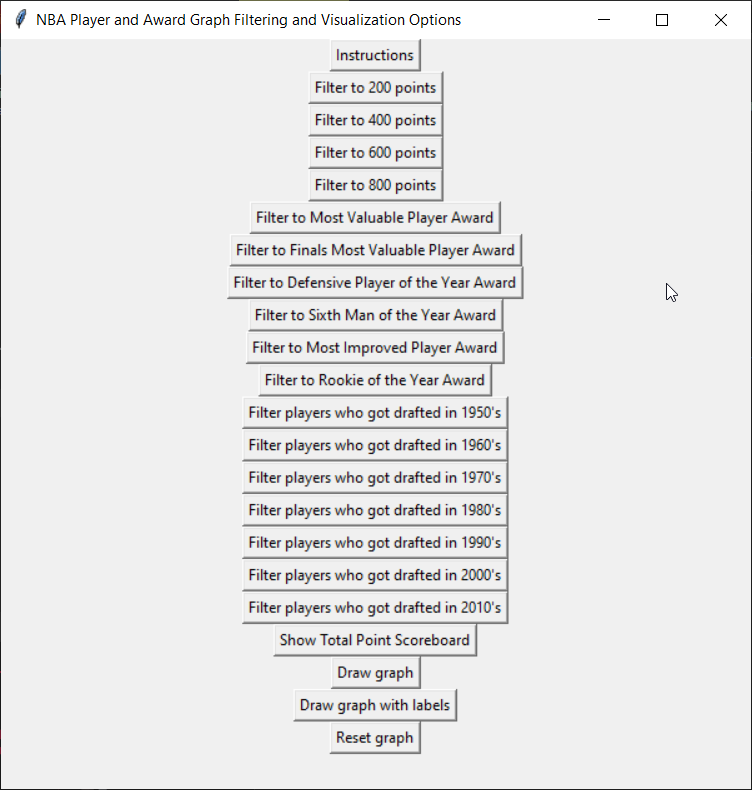
\includegraphics[width=18cm]{gui.png}
In this GUI, you will have many buttons but you should start with clicking the instructions button that will pop up another window to read. After reading this then you should have a good idea of how the GUI and program works. When you draw a graph, there should be another window that appears which displays the plot that you have just drawn, whether it was the original graph or a filtered version. This window can be expanded to get a better view of the graph. The new window with the graph visualization should look something like this (with PyCharm)\\
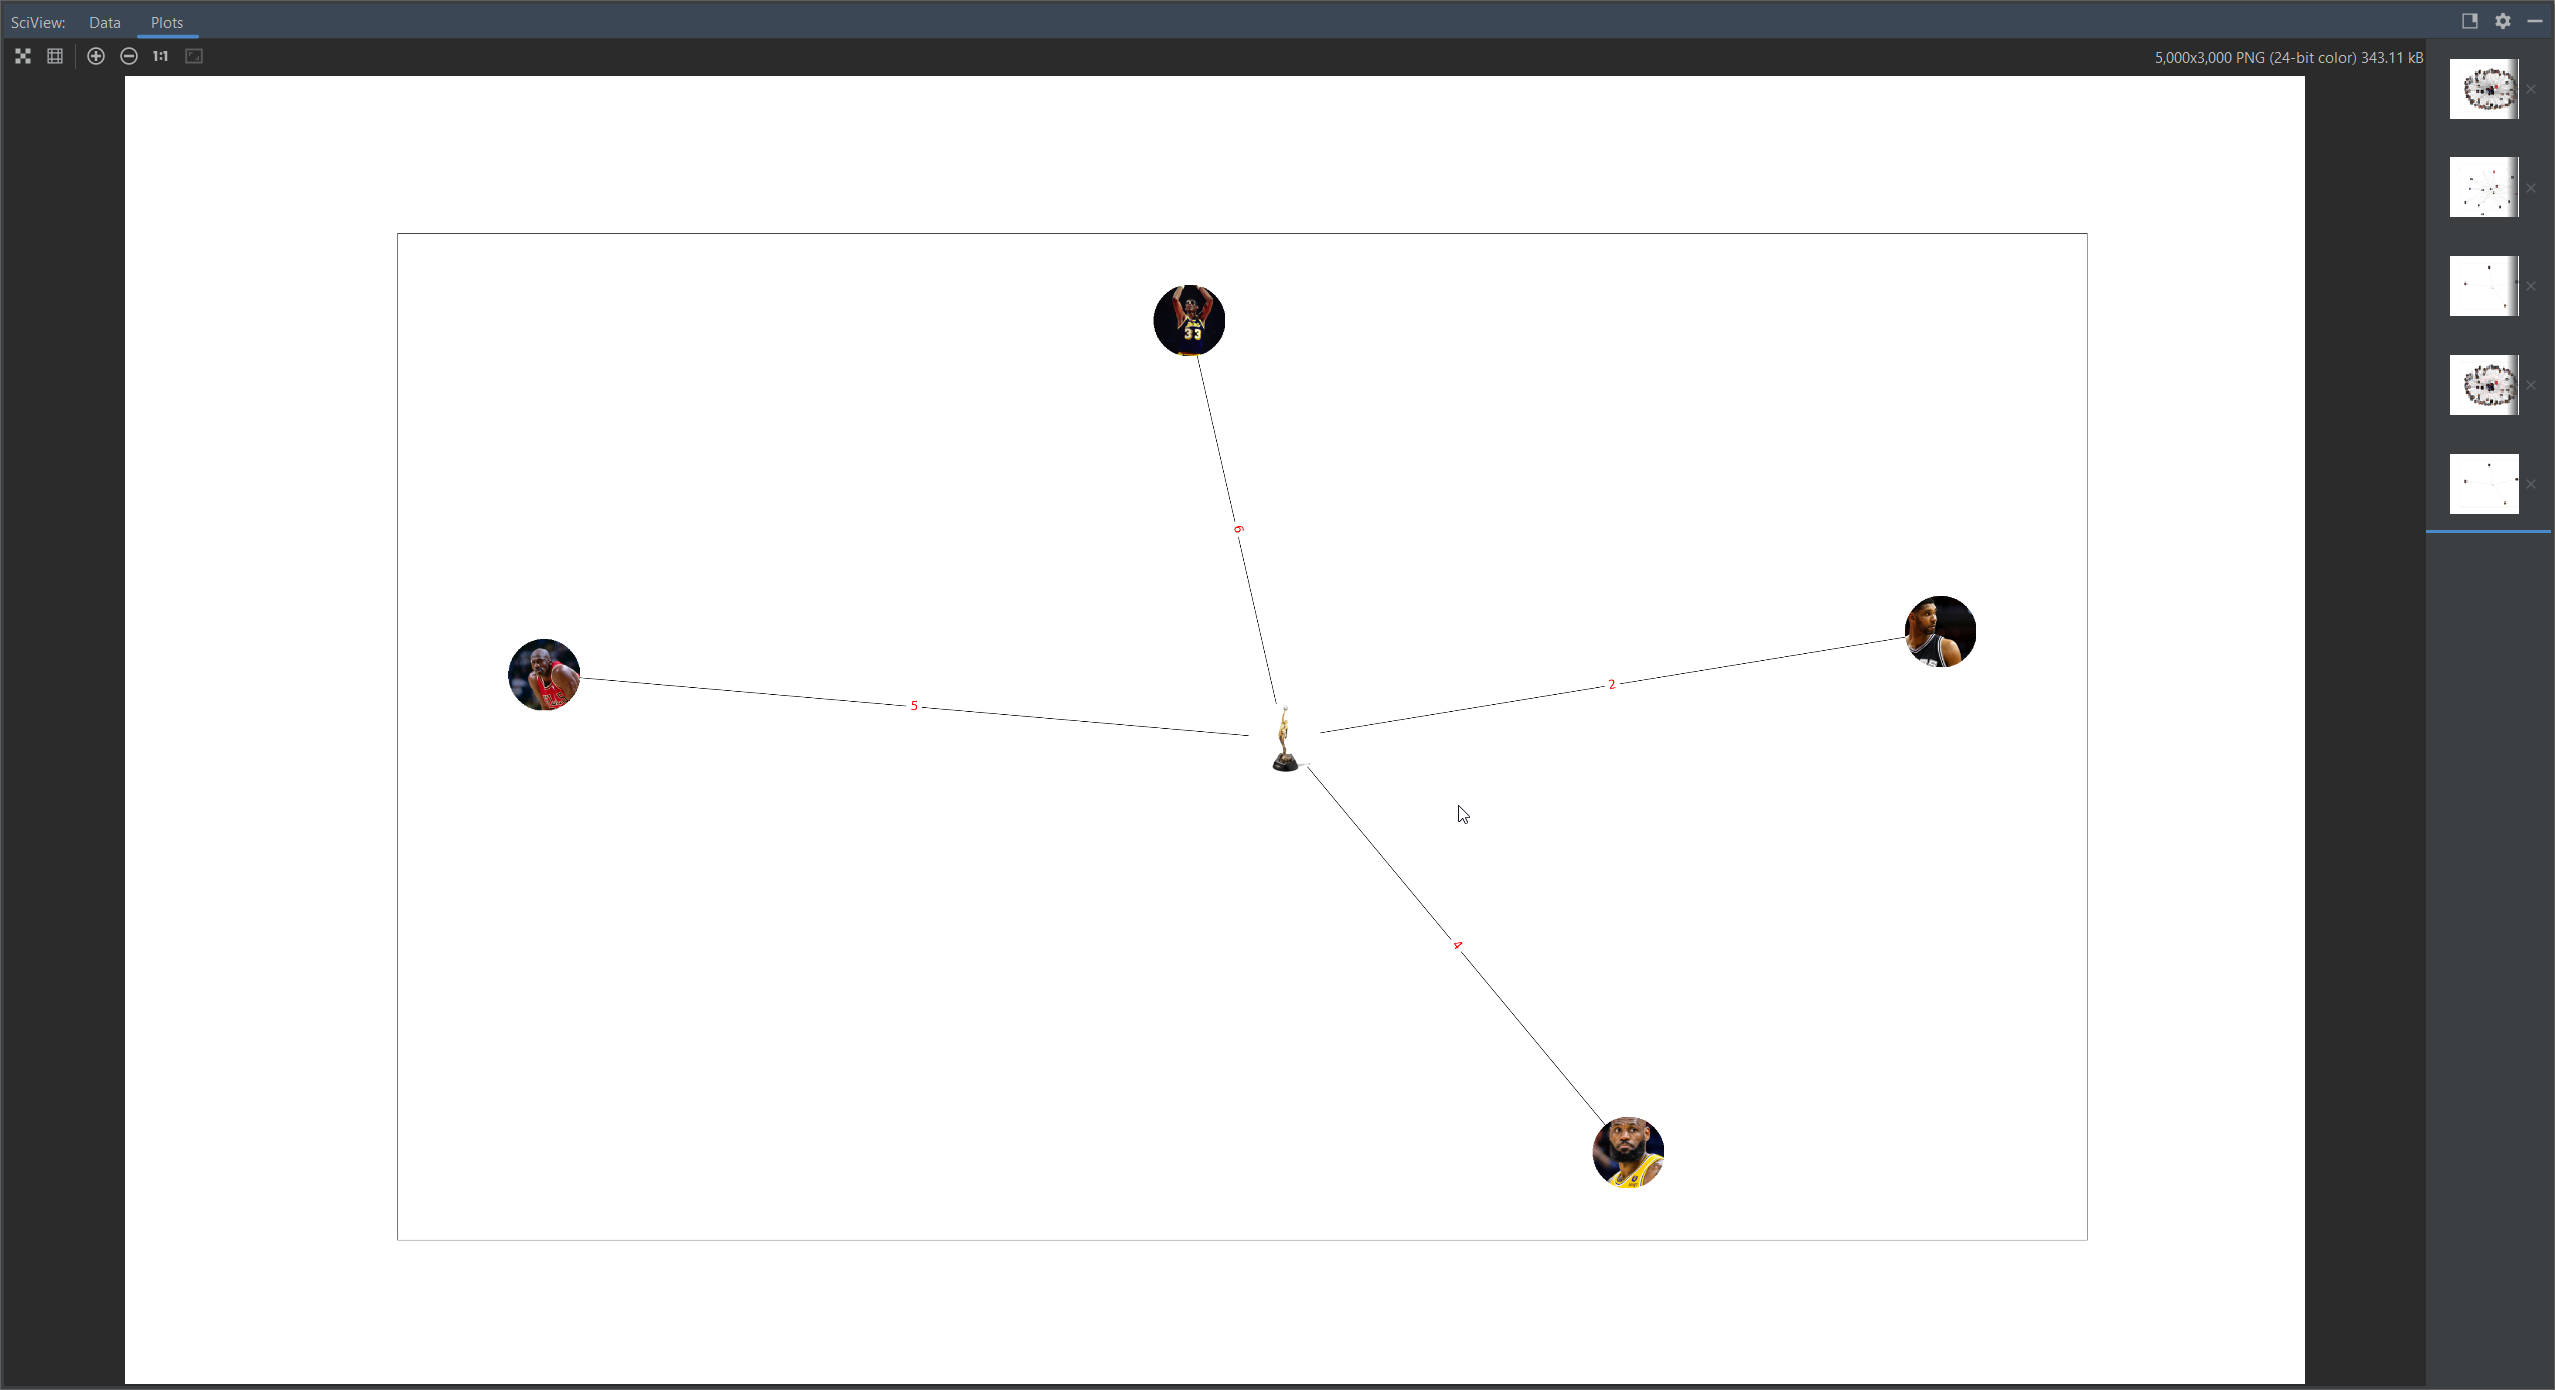
\includegraphics[width=18cm]{pycharmss.png}
Or this (using console):\\
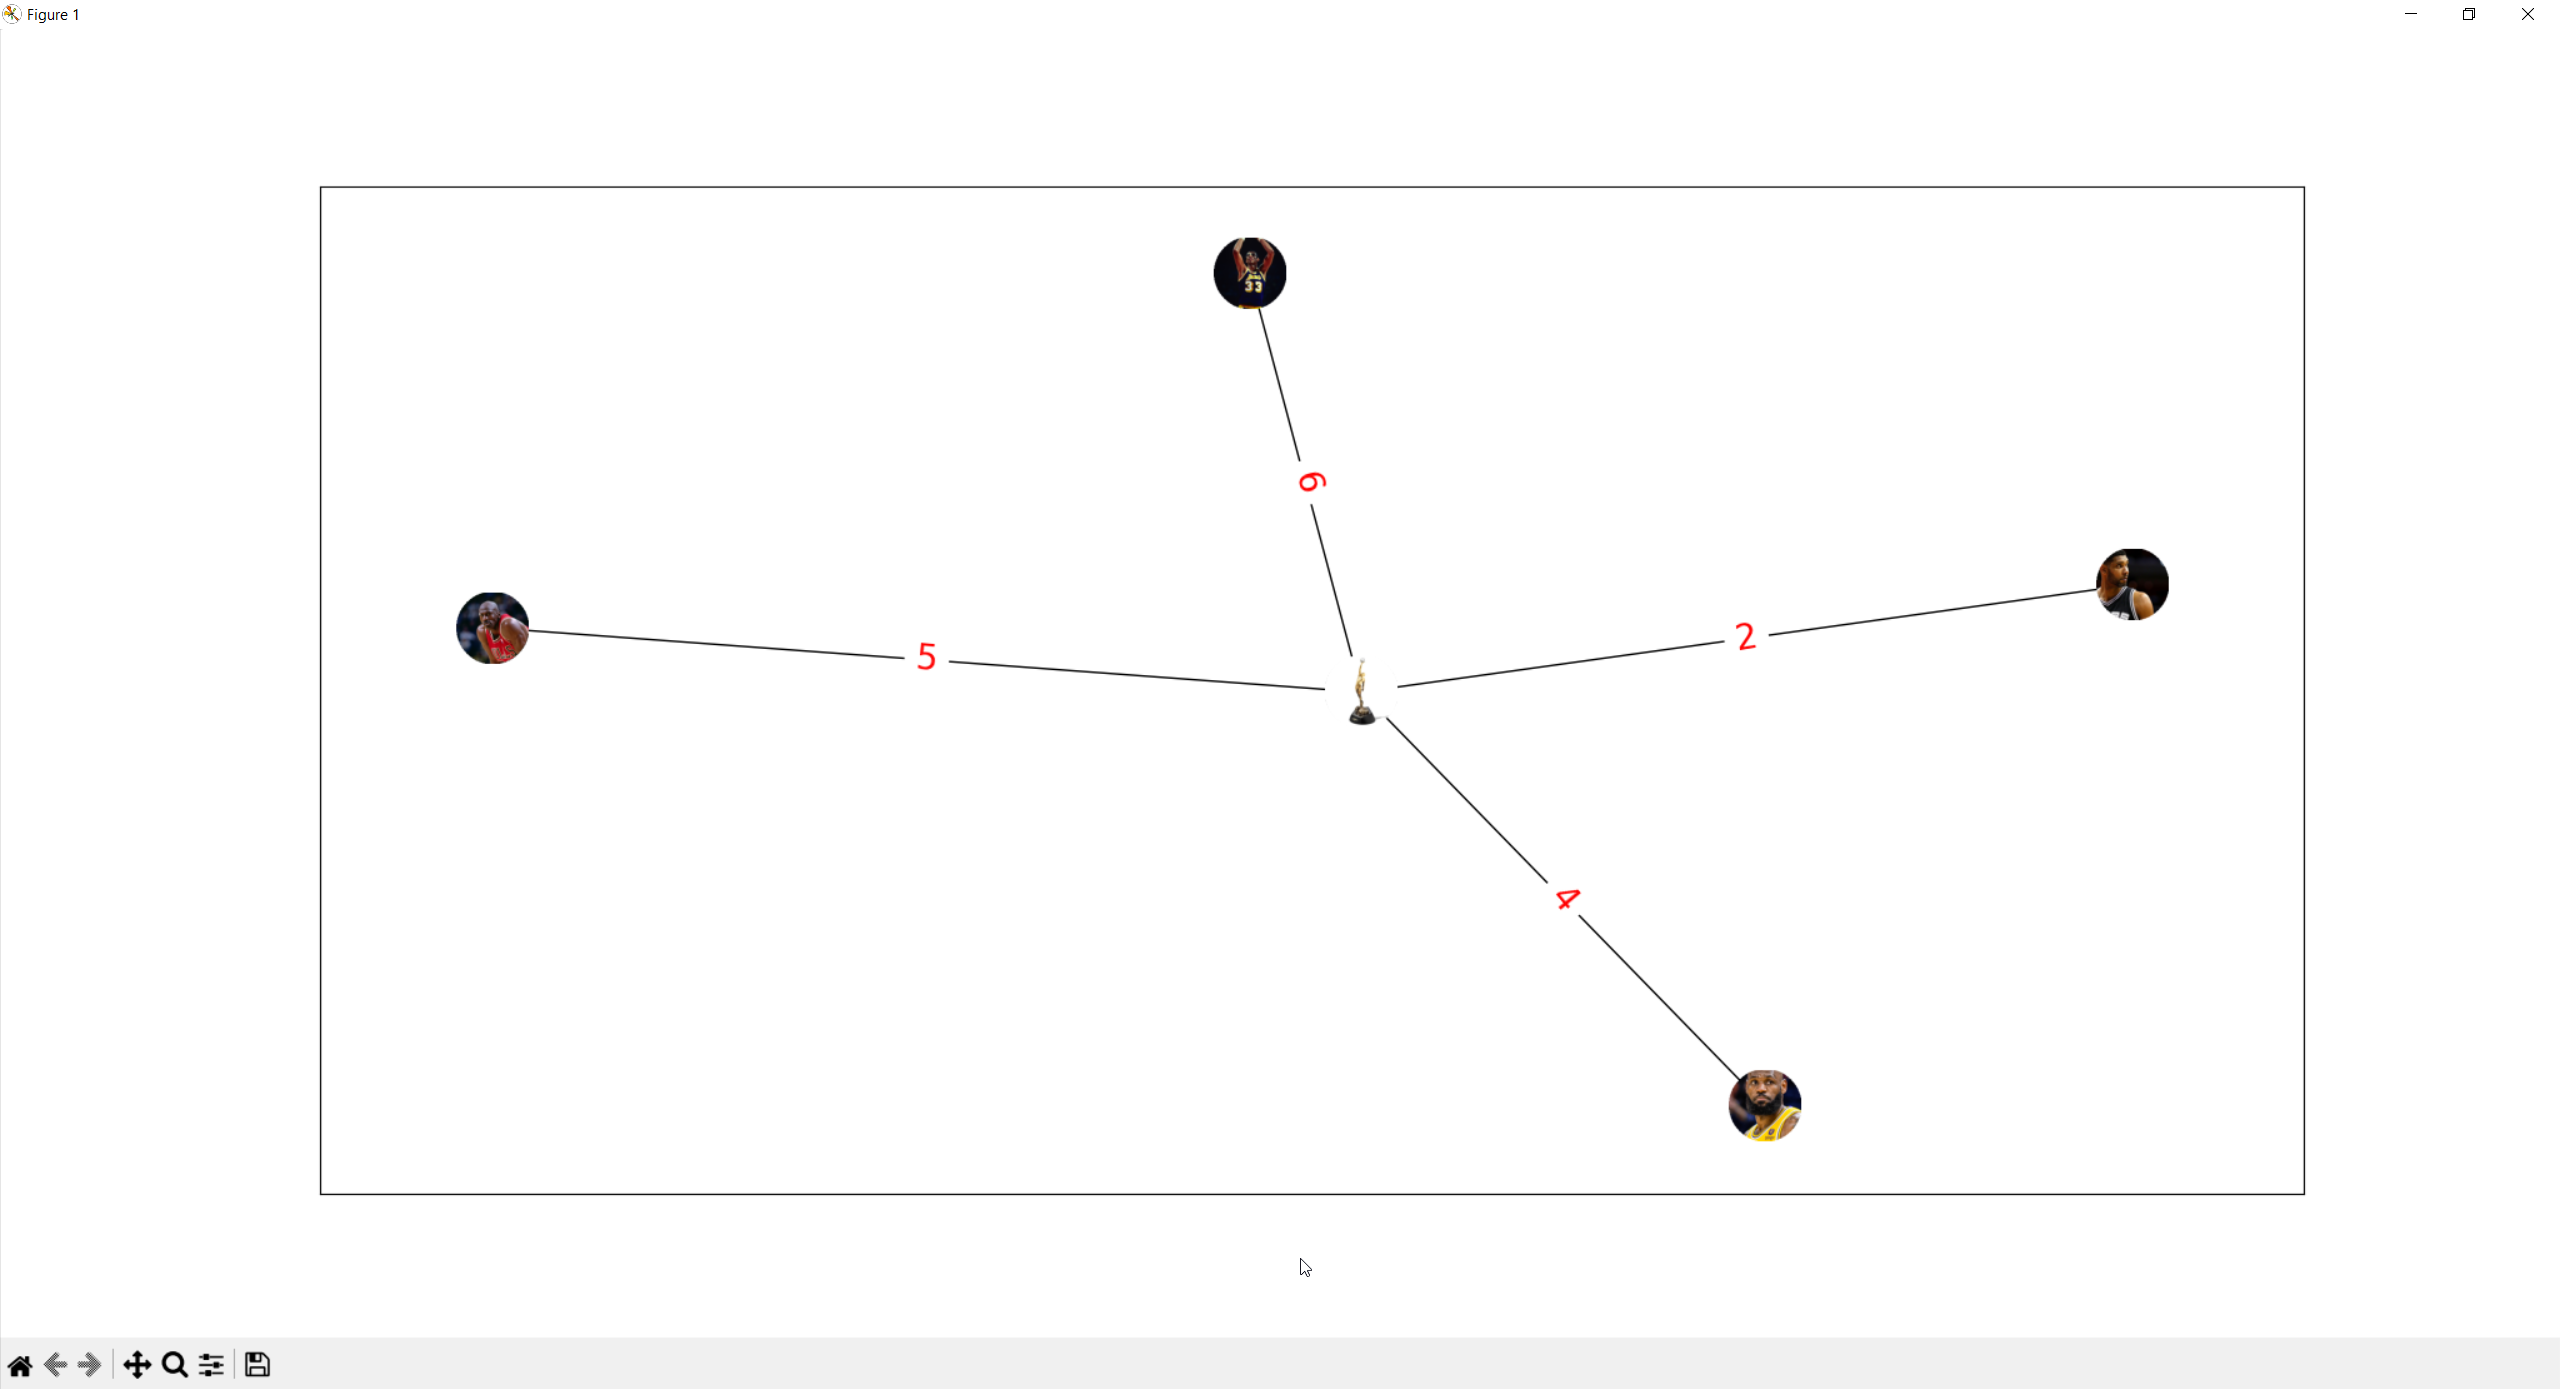
\includegraphics[width=18cm]{consoless.png}
You can experiment with the filters, keeping in mind the instructions provided in the GUI instruction message popup.

\section{Changes to the Project Plan}

Throughout the course of our project, several changes have been made to our initial plan in response to TA feedback, discussions with the instructor during office hours, and our own exploration of ideas. Here, we summarize the main changes we have made to our project since the initial proposal.

\subsection{Data Collection and Analysis}
In our initial proposal, we focused on analyzing game scores above 30. However, after considering the feedback and thinking about the amount of data required to generate meaningful insights, we feel the case with over 30 game scores is too extreme and can not give a clear insight into players performance. Thus, we decided to focus our analysis on season and history awards. This change allowed us to perform a more comprehensive analysis of player performance and better address our research questions.

\subsection{Libraries and Tools}
Based on the suggestions in the TA feedback, we have made changes to the libraries and tools we used for our project. We decided not to use Pandas, Pygame, or other libraries for data management, visualization, and interaction with users. Instead, we focused on using Python's built-in data structures and functionalities, as well as NetworkX, Plotly, and Matplotlib for generating visualizations and statistics.

\subsection{Bipartite Graphs}
We initially planned to create a graph with players and teams as nodes. After learning about stuff in tutorial 8, we realized that our graph was, in fact, a bipartite graph, with players and awards as nodes and achieved as edges. We incorporated this concept into our project, which helped us better understand and analyze the structure of the AwardNetwork.

\subsection{Interactive Visualization}
Although we considered using Tkinter or other libraries to create an interactive GUI, we ultimately decided to focus on a more static visualization approach using Plotly and Matplotlib. This allowed us to present the data in a clear and concise manner while still providing meaningful insights into player performance and awards record.

\subsection{Inline Citations}
Following the TA's advice, we have included inline citations in our final submission to provide proper attribution and context for the sources we used in our project.

These changes have strengthened our project by providing a more comprehensive analysis of NBA player performance and their achievements. By addressing the TA feedback and incorporating new ideas, we believe that our project now offers a deeper understanding of the relationships between players and their awards, and the role of these awards in shaping their careers.


\section{Discussion}

Our primary goal was to create an "AwardNetwork" that represents the connections between NBA players and their awards, allowing us to explore the relationships between players and their achievements throughout their careers. In this section, we discuss the results of our computational exploration, the limitations we encountered, and the potential next steps for further investigation.

\subsection{Results and Achievements}

The AwardNetwork we created using Python, NetworkX, and other libraries has provided a valuable tool for visualizing and analyzing the relationships between NBA players and their awards. By examining the AwardNetwork, we were able to address our initial research questions:

\begin{itemize}
\item We identified players with the most awards and compared their careers to others, revealing key differences in terms of achievements and career trajectories. Specifically, the top two players in all of NBA according to our points is Michael Jordan and Lebron James. Following relatively closely after those two is Kareem Abdul-Jabbar. We can deduce that these are the top three players in NBA history using awards, considering the gap between the top three players and the next player.
\item We discovered commonalities among players who have won specific awards, which could provide insights into the skills and attributes required to excel in particular aspects of the game. For example, the top three players, Michael Jordan, Lebron James and Kareem Abdul-Jabbar were all excellent at offense, able to score no matter the defender using their own signature moves. Michael Jordan was able to get a point from mid-range at will, Lebron James is unstoppable once he gets into the paint at full speed and Kareem Abdul-Jabbar was unguardable with his iconic sky-hook. All three players excelled at offence but all three also had impressive defensive skills and the longevity of Kareem and Lebron is extremely impressive. All these skills and attributes of these three players show the immense talent and skill needed to be at the top of the NBA.
\end{itemize}

Overall, the results of our computational exploration have helped us achieve our project goal and provided a deeper understanding of NBA player achievements.

\subsection{Limitations}

Despite our project's success, we encountered several limitations during our computational exploration:

\begin{itemize}
\item The dataset we used may not be comprehensive enough to capture the entire scope of NBA player achievements, as it only includes the top 75 players and their awards.
\item We relied on NetworkX, Plotly, and Matplotlib for visualizations, which, while effective, may not offer the most advanced or interactive visualization options available.
\item Our analysis focused on the relationships between players and awards, but we did not dive into other potentially relevant factors, such as player positions, team dynamics, or the impact of coaching staff.
\item The dataset was relatively large and because of this, the visualizations were not as good as we wanted them to be with the nodes being very tightly packed together and many edges, making it hard to see which player links to which award. Fortunately, we were able to make filtering for our graph but the visualizations still are not as good as we would want them to be.
\end{itemize}

\subsection{Next Steps}

To further enhance our project, several next steps could be explored:

\begin{itemize}
\item Expand the dataset to include a more comprehensive list of players and awards, allowing for a more thorough analysis of player achievements across the NBA.
\item Implement advanced interactive visualizations using libraries like D3.js or Plotly Dash to provide users with a more engaging and informative experience.
\item Incorporate additional variables, such as player positions, team dynamics, and coaching staff, to gain a more holistic understanding of the factors that contribute to player achievements.
\item Utilize machine learning algorithms to predict future award winners based on historical data and player performance metrics.
\end{itemize}

\subsection{Conclusion}

In conclusion, our project successfully created an AwardNetwork that visualizes and analyzes the relationships between NBA players and their awards. Although we encountered some limitations, our computational exploration has provided valuable insights into player achievements and the role of awards in shaping their careers. By pursuing the next steps outlined above, we can further enhance our understanding of NBA player performance and continue to contribute to the broader study of professional sports achievements.


\section{References}

\begin{tabular}{@{}p{0.5cm}p{14cm}@{}}
    [1] & RealGM, "Michael Jordan Awards," RealGM, 2023. [Online]. \\
        & Available: \url{https://basketball.realgm.com/nba/awards/by_player}. \\
        & [Accessed: April 2, 2023]. \\
\end{tabular}




% NOTE: LaTeX does have a built-in way of generating references automatically,
% but it's a bit tricky to use so we STRONGLY recommend writing your references
% manually, using a standard academic format like APA or MLA.
% (E.g., https://owl.purdue.edu/owl/research_and_citation/apa_style/apa_formatting_and_style_guide/general_format.html)

\end{document}